\section{EKSPERIMENTAI}
\label{eksperimentai}

Šiame skyriuje yra aprašyti eksperimentuose naudoti biomedicininių duomenų rinkiniai, įvardinti eksperimentų nustatymai, pateikti matų atrinkimo metodų spartos matavimai, pristatyti klasifikavimo tikslumo matavimai ir apžvelgti stabilių matų atrinkimo rezultatai. 

\subsection{Eksperimentuose naudoti duomenys}
\label{eksperimentuose_naudoti_duomenys}

Šiame darbe eksperimentai buvo atliekami su biomedicininiais viešai prieinamais genų ekspresijos mėginių rinkiniais. Informacija apie mėginių rinkinius pateikta \ref{table:datasets} lentelėje.
\begin{longtable}{|p{4.5cm}|p{2cm}|p{3.5cm}|p{2.3cm}|p{2cm}|}
\captionsetup{labelsep=period}
\caption{Darbe naudoti mėginių rinkiniai\label{table:datasets}}\\
%This is the header for the first page of the table...
\hline \hline
{\textbf{Pavadinimas}} &
{\textbf{Šaltinis}} &
{\textbf{Mėginių skaičius (+/-)}} &
{\textbf{Matų \newline skaičius}} &
{\textbf{OMS}}\\
\hline
\endfirsthead
%This is the header for the remaining page(s) of the table...
\multicolumn{3}{c}{{\tablename} \thetable{} -- Tęsinys} \\[0.5ex]
\hline \hline
{\textbf{Pavadinimas}} &
{\textbf{Šaltinis}} &
{\textbf{Mėginių skaičius (+/-)}}&
{\textbf{Matų \newline skaičius}} &
{\textbf{OMS}}\\
\hline
\endhead
%This is the footer for all pages except the last page of the table...
\multicolumn{3}{l}{{Lentelės tęsinys kitame puslapyje\ldots}} \\
\endfoot
%This is the footer for the last page of the table...
\hline \hline
\endlastfoot
\hline 
Gaubtinės žarnos auglys (angl. Colon) 
& 
\cite{alon1999broad} 
& 
62 (40/22) 
& 
2000 
& 
0.031 \\
\hline
Centrinės nervų sistemos auglys (CNS) 
& 
\cite{pomeroy2002prediction} 
& 
60 (39 / 21) 
& 
7129 
& 
0.0084 \\
\hline
Prostatos auglys 
& 
\cite{singh2002gene} 
& 
102 (52/50) 
& 
6033 
& 
0.0169 \\
\hline
Šizofrenija ir maniakinė depresija
&
\cite{altara}
&
90 \newline (bp\footnote{bp (angl. \textit{Bipolar Disorder}) - maniakine depresija sergantys pacientai.}:
sz\footnote{sz (angl. \textit{Schizophrenia}) - šizofrenija sergantys pacientai.}:
cc\footnote{cc (angl. \textit{Control Crowd}) - kontrolinė grupė.} \newline =30:31:29)
&
22283
&
0.00404 \\
\hline
\end{longtable}

Mėginių rinkinius apibūdinantis dydis OMS (Objektų-Matų Santykis), kuris turimiems mėginių rinkiniams yra nuo 0,403\% iki 3,01\% procento, reiškia, kad turimi mėginiai turi šimtus kartų daugiau matų nei mėginių. Tai apsunkina duomenų tyrimo procesą ir gali sukelti persimokymo (angl. \textit{overfitting}) problemą.

Šizofrenijos ir maniakinės depresijos mėginių rinkinys ypatingas tuo, kad jis turi tris klases. Šiame darbe nagrinėjamas tik dviejų klasių atvejis, todėl šizofrenija sergančių pacientų mėginiai nebuvo naudojami.

\subsection{Metodologija}

Eksperimentuose buvo naudojami skyrelyje nr. \ref{eksperimentuose_naudoti_duomenys}. aprašyti mėginių rinkiniai. Mėginių rinkiniai nebuvo atskirai normalizuojami, nes daryta prielaida, jog duomenys jau yra apdoroti. 

Klasifikavimui naudota atraminių vektorių klasifikatorių algoritmo R programavimo kalbos paketo ,,e1071`` implementacija. Naudotas tiesinis atraminių vektorių klasifikavimo algoritmas su parametro $C$ reikšme 0,01, kuri buvo nustatyta empiriškai.

Matų atrinkimo metodai buvo suprogramuoti šio darbo autoriaus, nes nėra standartinių R kalbos paketų, kuriuose matų atrinkimo metodai jau būtų implementuoti.

Dėl to, kad turima mažai mėginių ir daug matų, klasifikavimas buvo kartojamas 300 kartų, kai treniravimosi duomenų aibę sudarė kaskart atsitiktinai parenkami 90\% mėginių. Kiekvienoje iteracijoje su vis kitu mėginių poaibiu buvo atliekamas matų atrinkimas, po to būdavo atliekamas klasifikavimas su 10, 20, .., 500 aukščiausią reitingą turinčių matų.

\subsection{Matų atrinkimo metodų sparta}

Matų atrinkimo metodų darbo laikas buvo palygintas naudojant vieną biomedicininių duomenų rinkinį -- AltarA \cite{altara}. Skaičiavimai buvo atlikti kompiuteryje naudojant vieną procesoriaus branduolį veikiantį 2.66 GHz, bei 2 GB RAM atminties. \ref{fig:visu_laikas} pav. ir \ref{fig:cgs_laikas} pav. pavaizduota matų atrinkimo metodo darbo laiko priklausomybė nuo mėginius apibūdinančių matų skaičiaus. 
\begin{figure}[hq]
\begin{minipage}[b]{0.5\linewidth}
\centering
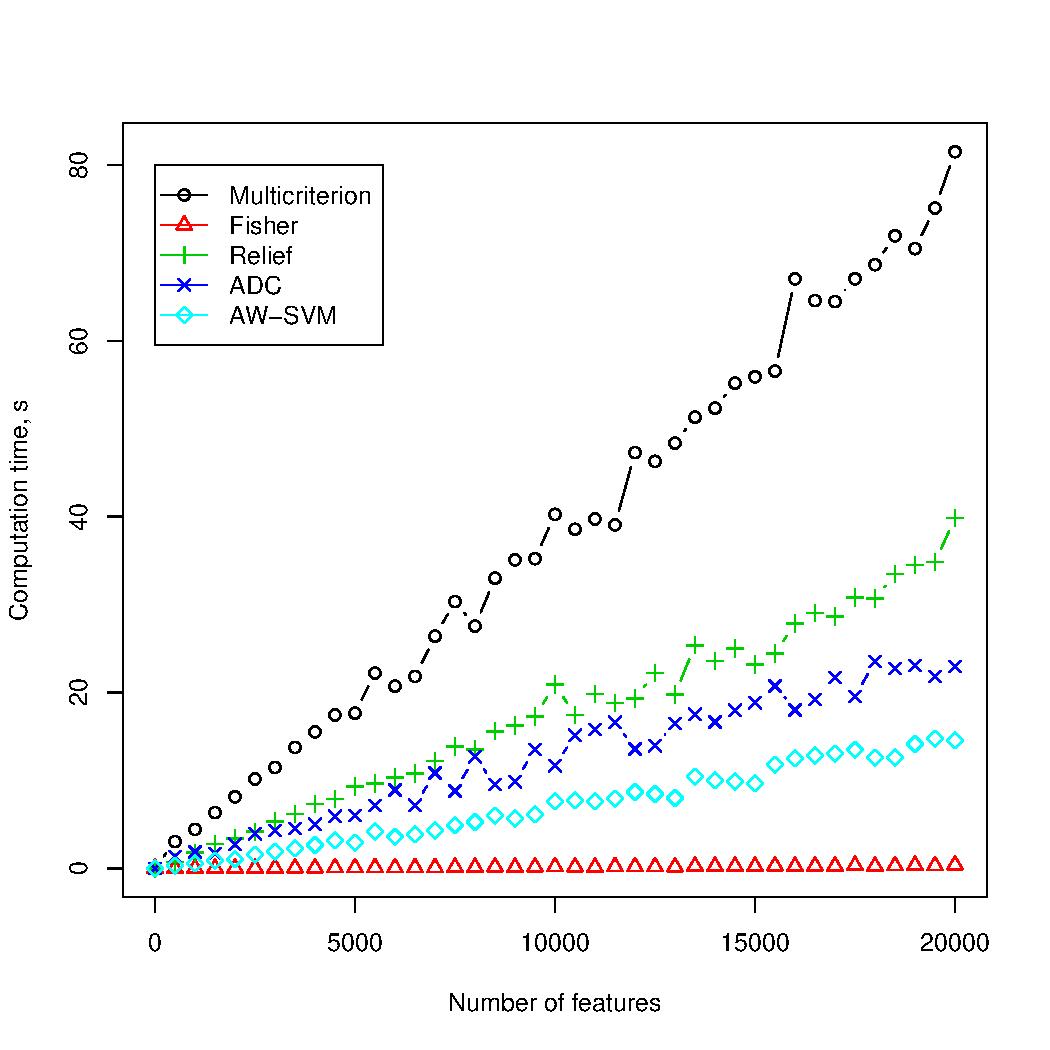
\includegraphics[width=1\textwidth]{images/all_performance.pdf}
 \caption{Pagrindinių matų atrinkimo metodų darbo laikas.}
 \label{fig:visu_laikas}
\end{minipage}
\hspace{0.2cm}
\begin{minipage}[b]{0.5\linewidth}
\centering
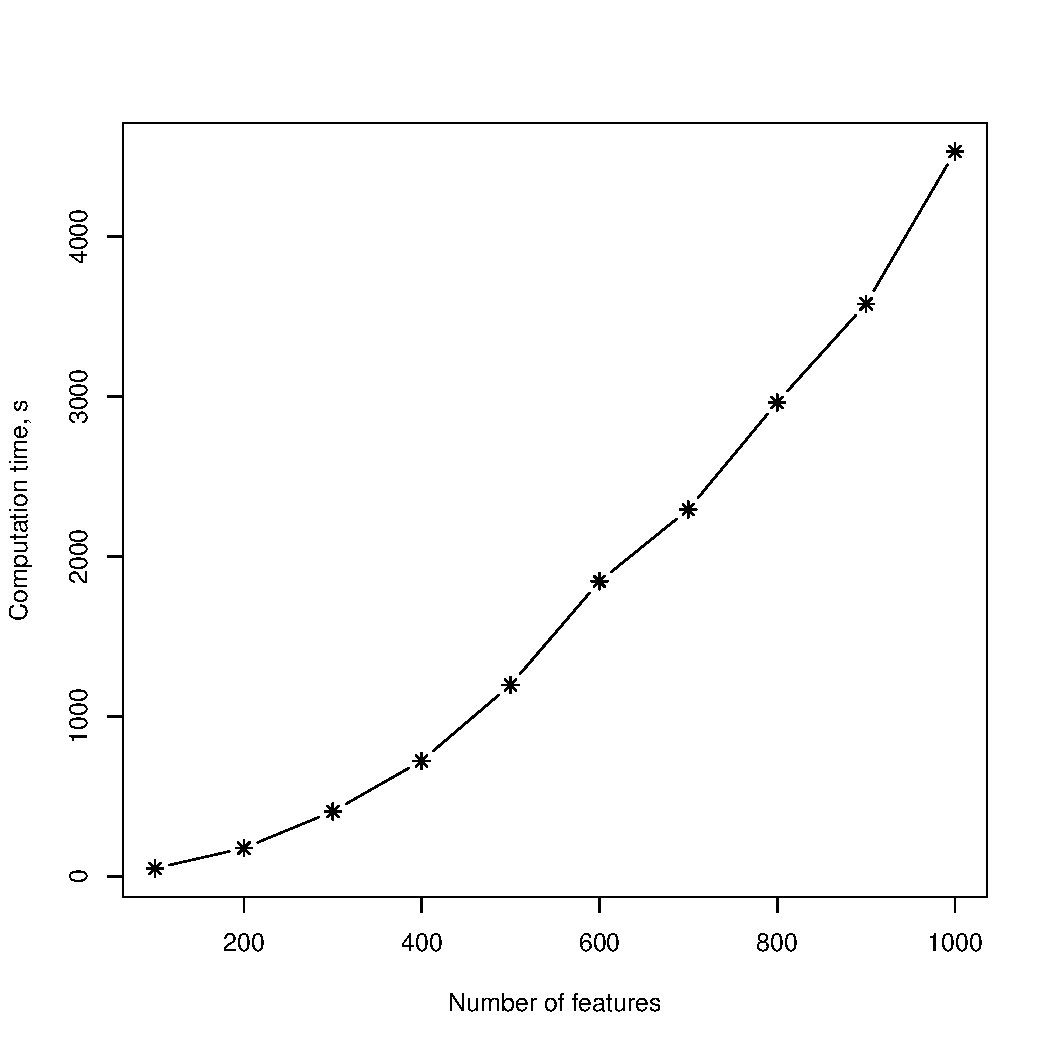
\includegraphics[width=1\textwidth]{images/cgs_performance.pdf}
 \caption{Konsensuso grupėmis grįsto matų atrinkimo metodo darbo laikas.}
 \label{fig:cgs_laikas}
\end{minipage}
\end{figure}

Matų atrinkimo metodų darbo laikas yra atvaizduotas dviem grafikais, nes pagal atliktų eksperimentų rezultatus buvo pastebėta, kad CGS matų atrinkimo metodas yra apie 1000 kartų lėtesnis už kitus suprogramuotus matų atrinkimo metodus, todėl viename grafike neįmanoma atvaizduoti visų turimų matų atrinkimo metodų. Pagal \ref{fig:visu_laikas} pav. galime daryti išvadą, kad sparčiausias matų atrinkimo metodas yra \textit{Fisher} įvertis. Remiantis matų darbo laiko priklausomybės nuo matų kiekio grafikais galime daryti išvadą, kad CGS algoritmas daugiamačių duomenų matų atrinkimui nėra tinkamas, nes jo skaičiavimų laikas yra per ilgas.

\subsection{Klasifikavimo pagal atrinktus matus tikslumas}

Matų atrinkimo metodų įtaką klasifikavimo klasifikavimo tikslumui buvo matuojama naudojant tris biomedicininių duomenų rinkinius: gaubtinės žarnos auglio (angl. \textit{colon}), centrinės nervų sistemos (CNS), prostatos. Klasifikavimui buvo naudojami tiesiniai atraminių vektorių klasifikatoriai (SVM), su empiriškai nustatytu parametru $C=0.01$. Keičiant parametrus keičiasi ir klasifikavimo tikslumas.
Klasifikatoriui apmokyti buvo naudojama 90\% atsitiktinai parinktų mėginių iš duomenų rinkinio. Likusiais 10\% mėginių buvo testuojamas klasifikatorius. Klasifikatorius buvo testuojamas po 300 kartų su įvairiu matų skaičiumi: nuo 10 iki 500. Klasifikavimo tikslumas pavaizduotas dviejų tipų grafikais: klasifikavimo nuostolio priklausomybės nuo atrinktų matų skaičiaus, bei ROC kreivėmis, kurios buvo apskaičiuotos pagal duomenis gautus klasifikuojant su tiek atrinktų matų, su kiek klasifikavimo tikslumas buvo pats geriausias \cite{green1966signal}.
\begin{figure}[H]
\begin{minipage}[b]{0.5\linewidth}
\centering
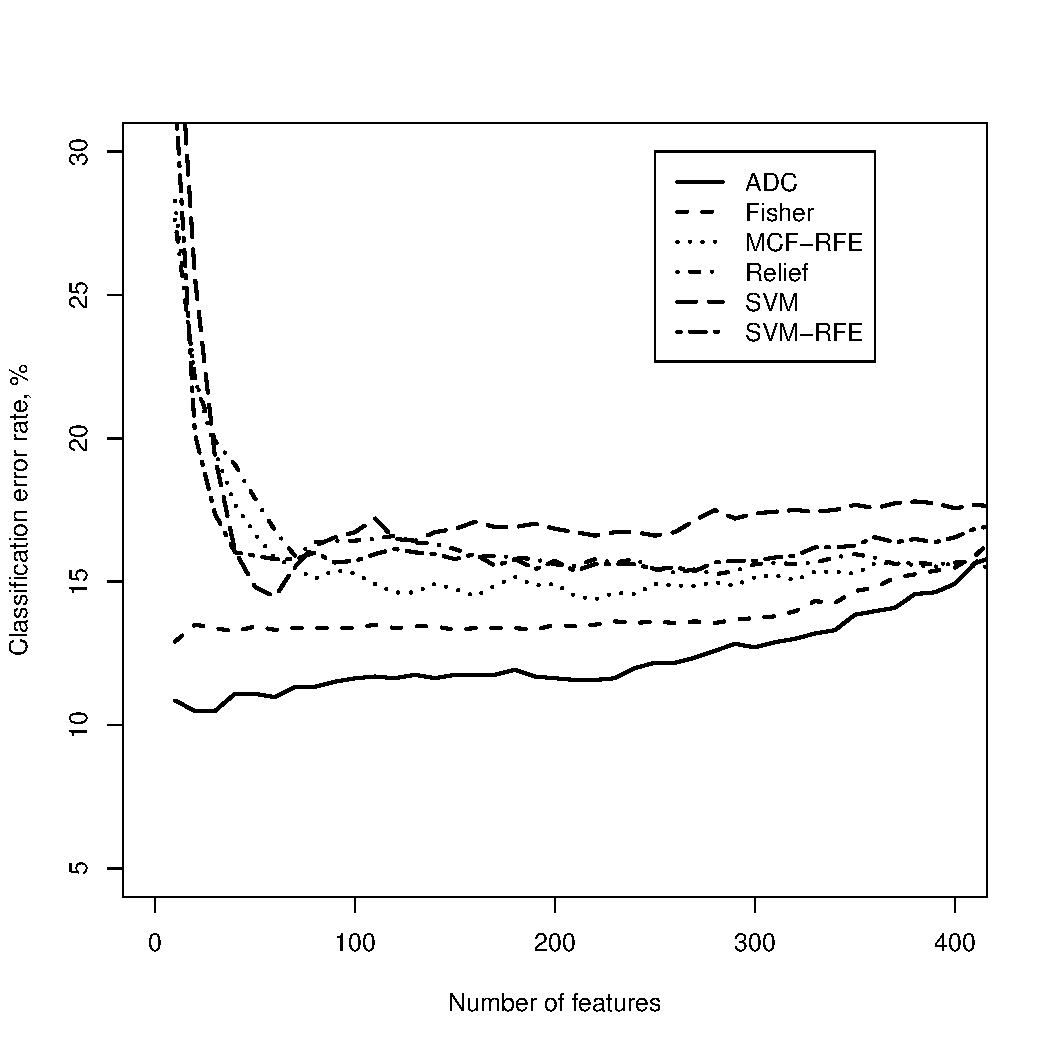
\includegraphics[width=0.9\textwidth]{../bachelor/images/nncolon_classification.pdf}
\caption{Gaubtinės žarnos auglio meginių klasifikatorių tikslumas.}
\label{fig:class_colon}
\end{minipage}
\hspace{0.2cm}
\begin{minipage}[b]{0.5\linewidth}
\centering
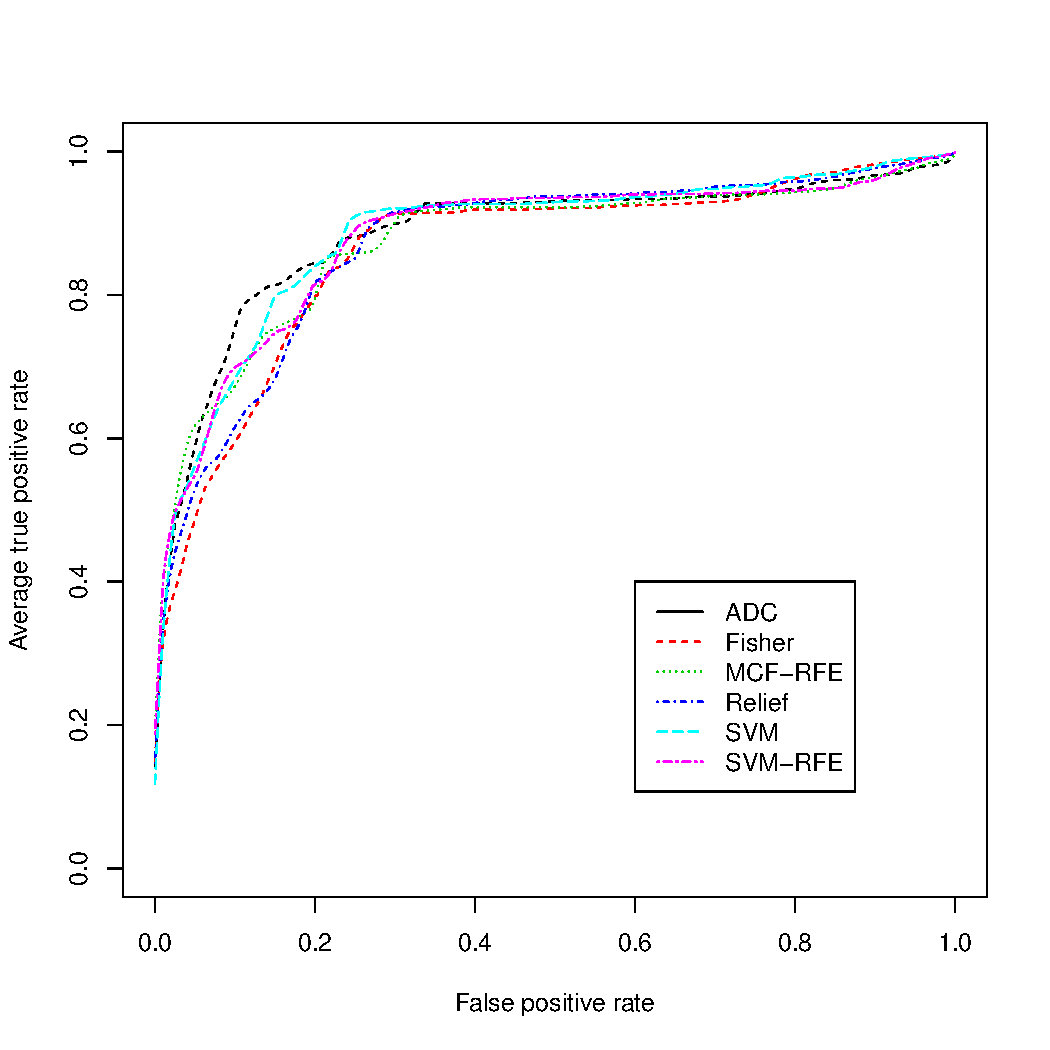
\includegraphics[width=0.9\textwidth]{../bachelor/images/nncolon_roc.pdf}
\caption{Gaubtinės žarnos auglio mėginių klasifikatorių ROC kreivės.}
\label{fig:roc_colon}
\end{minipage}
\hspace{0.2cm}
\begin{minipage}[b]{0.5\linewidth}
\centering
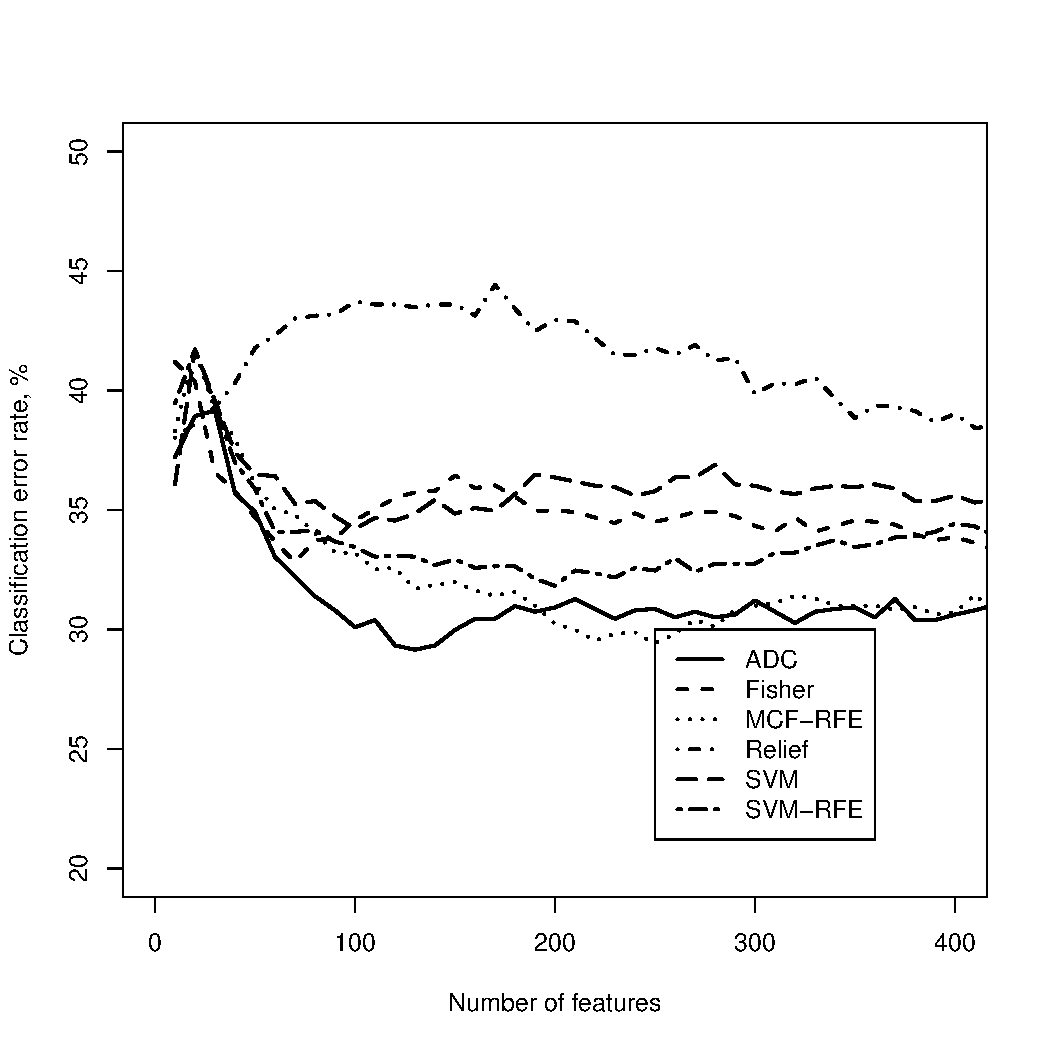
\includegraphics[width=.9\textwidth]{../bachelor/images/nncns_classification.pdf}
\caption{Centrinės nervų sistemos meginių klasifikatorių tikslumas.}
\label{fig:class_cns}
\end{minipage}
\hspace{0.2cm}
\begin{minipage}[b]{0.5\linewidth}
\centering
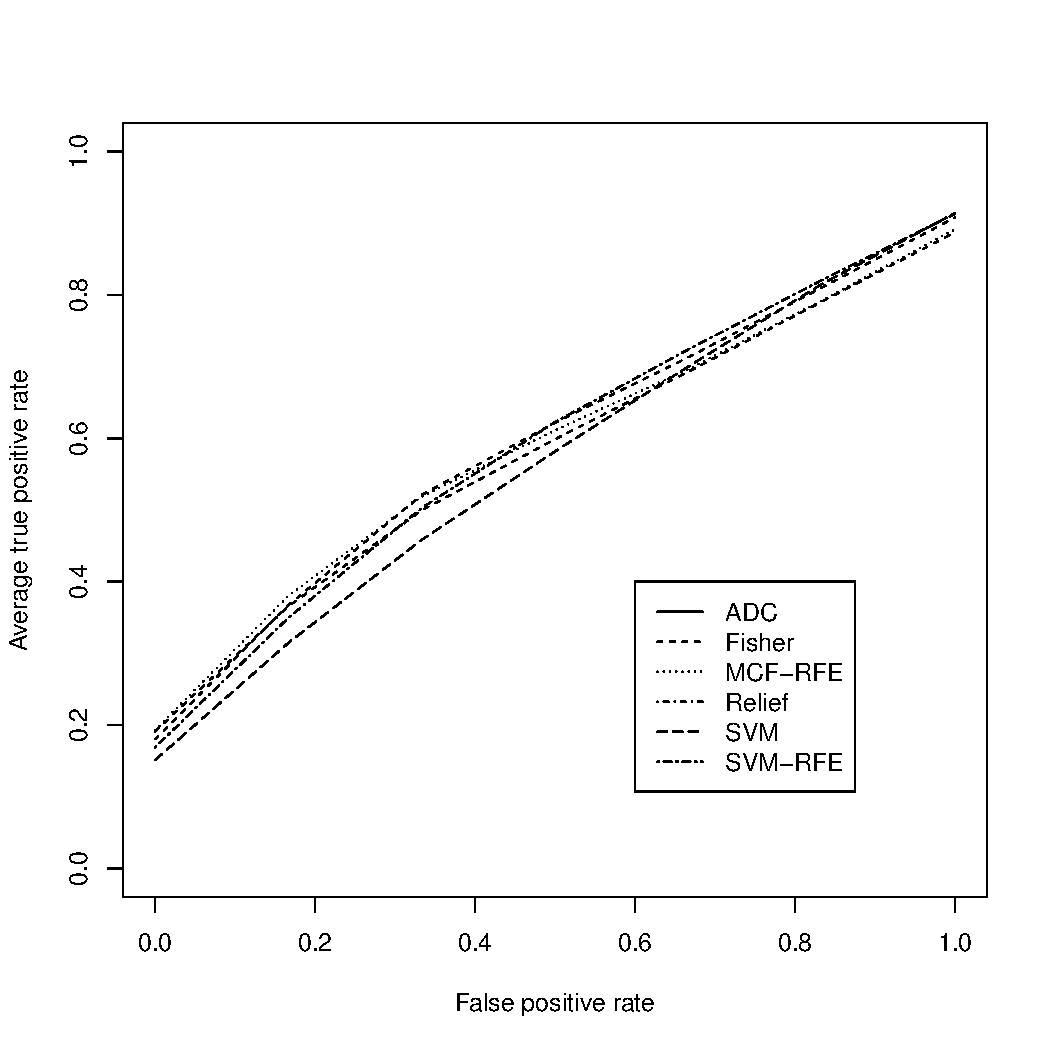
\includegraphics[width=.9\textwidth]{../bachelor/images/nncns_roc.pdf}
\caption{Centrinės nervų sistemos mėginių klasifikatorių ROC kreivės.}
\label{fig:roc_cns}
\end{minipage}
\hspace{0.2cm}
\begin{minipage}[b]{0.5\linewidth}
\centering
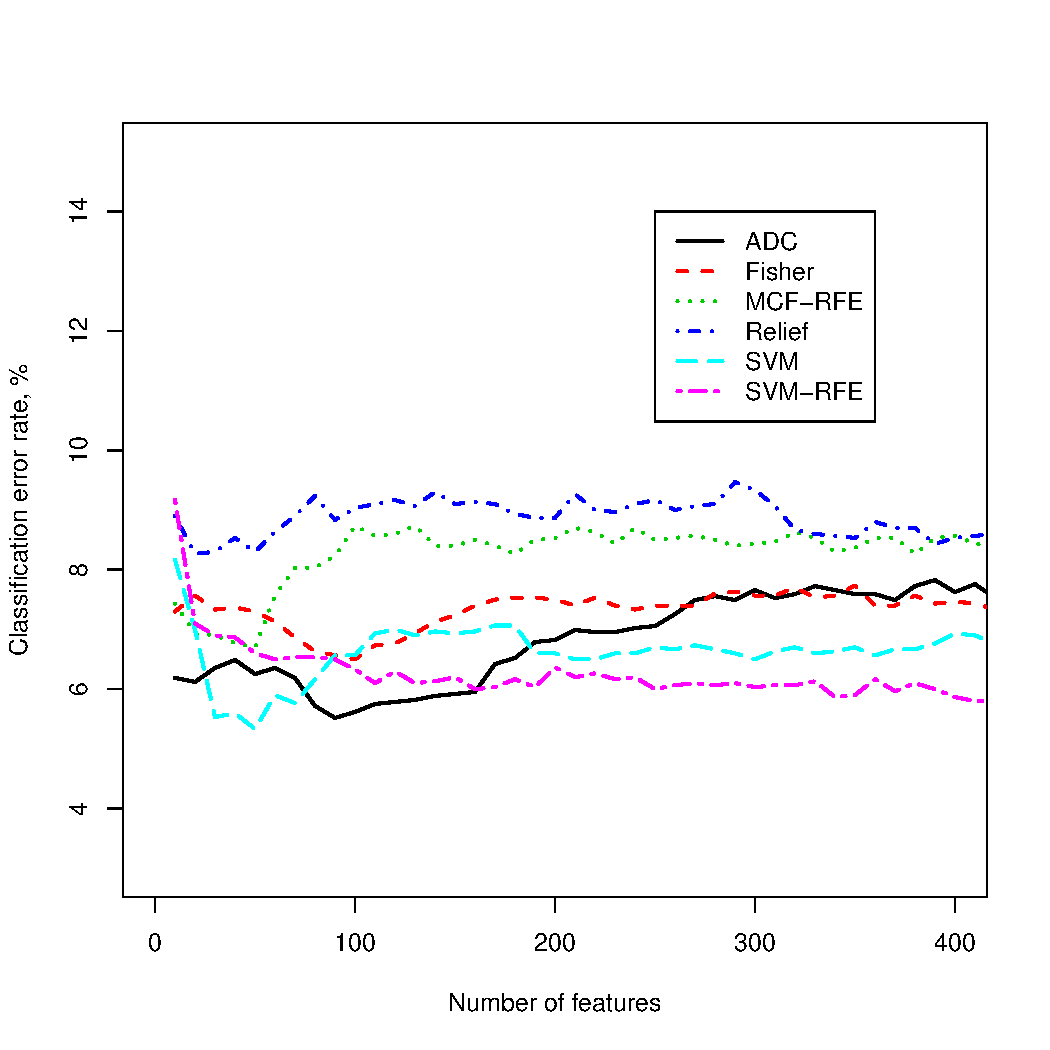
\includegraphics[width=.9\textwidth]{../bachelor/images/prostate_classification.pdf}
\caption{Prostatos meginių klasifikatorių tikslumas.}
\label{fig:class_prostate}
\end{minipage}
\hspace{0.2cm}
\begin{minipage}[b]{0.5\linewidth}
\centering
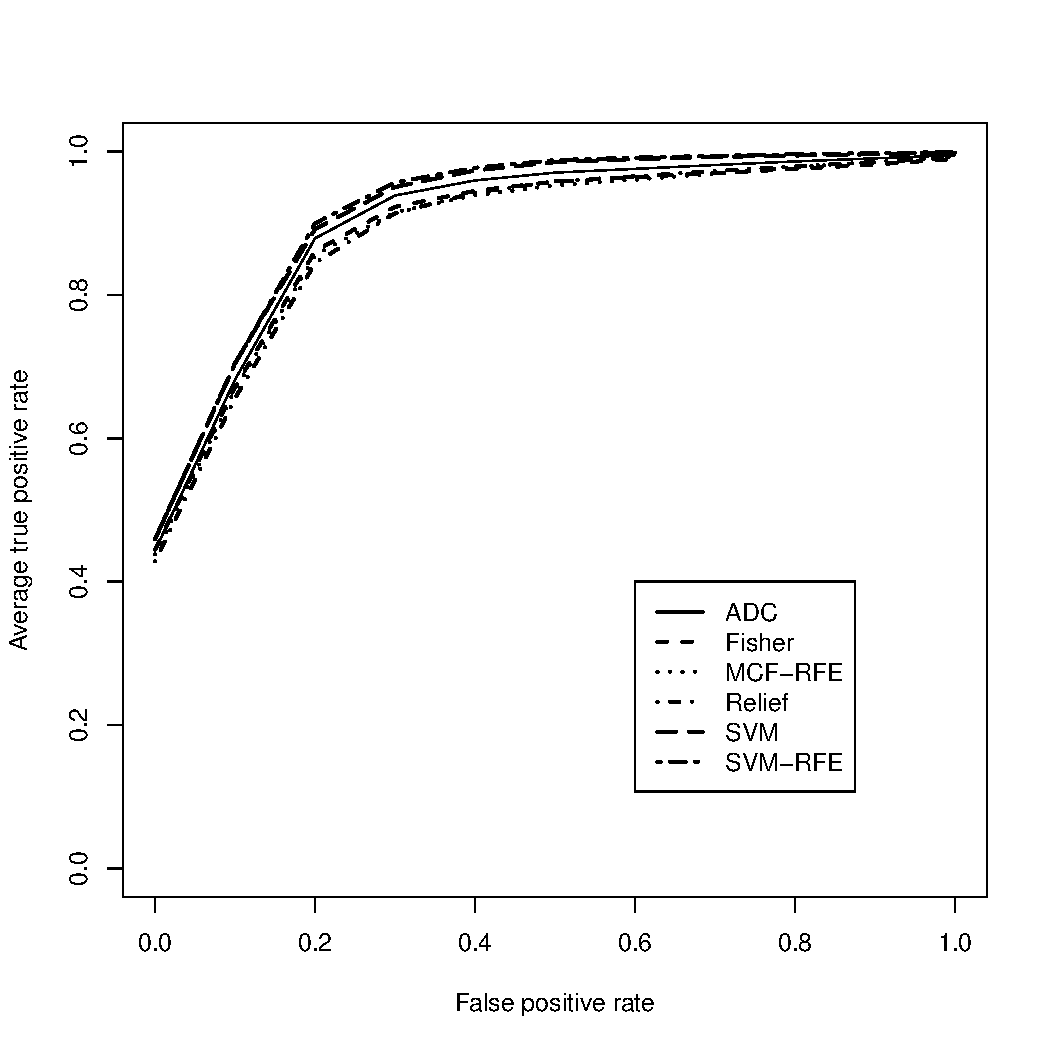
\includegraphics[width=.9\textwidth]{../bachelor/images/prostate_roc.pdf}
\caption{Prostatos mėginių klasifikatorių ROC kreivės.}
\label{fig:roc_prostate}
\end{minipage}
\end{figure}
\ref{fig:class_colon} pav. matome, kad gaubtinės žarnos auglio duomenų rinkinio matus geriausiai atrenka ADC metodas. Tik šiek tiek prasčiau pasirodo \textit{Fisher} įvertis. Blogiausiai su gaubtinės žarnos auglio mėginiais susidoroja absoliučių svorių SVM matų atrinkimo metodas.

Centrinės nervų sistemos duomenų rinkinys yra sunkiai klasifikuojamas, nes vidutinis klaidų skaičius yra apie 35\%, kai, pvz. gautinės žarnos auglio duomenų rinkinio vidutinis klaidų skaičius yra tik 15\%. \ref{fig:class_cns} pav. matome, kad šiam duomenų rinkiniui vidutiniškai geriausiai matus atrenka ADC ir multikriterinio rekursyvaus matų eliminavimo metodai. Prasčiausiai pasirodo \textit{Relief} metodas.
\ref{fig:class_prostate} pav. parodyta, kad prostatos duomenų rinkinio matus klasifikavimui geriausiai atrenka ADC bei absoliučių svorių SVM metodas. Prasčiausiai matus atrenka \textit{Relief}.

Apibendrindamas gautus klasifikavimo tikslumo matavimo rezultatus, galiu teigti, kad nėra vieno absoliučiai geriausio matų atrinkimo metodo. Reikia eksperimentuoti, kad būtų rastas konkrečiai problemai geriausiai tinkantis matų atrinkimo metodas. Tačiau rezultatai parodė, kad matų atrinkimas svariai prisideda prie geresnio klasifikatoriaus sukūrimo.

\subsection{Matų atrinkimo stabilumas}

Matų atrinkimo stabilumas buvo tiriamas naudojant tuos pačius biomedicininių duomenų rinkinius kaip ir tiriant klasifikavimo pagal atrinktus matus tikslumą. Matų atrinkimo stabilumas buvo matuojamas pagal \textit{Kuncheva} ir \textit{Jaccard} indeksus. Stabilumas pats savaime nėra svarbus, jis turi būti matuojamas atsižvelgiant į klasifikavimo tikslumą. Todėl šio poskyrio grafikus reikia nagrinėti atsižvelgiant į poskyrio, kuriame buvo nagrinėtas klasifikavimo pagal atrinktus matus tikslumas.

\begin{figure}[H]
\begin{minipage}[b]{0.47\linewidth}
\centering
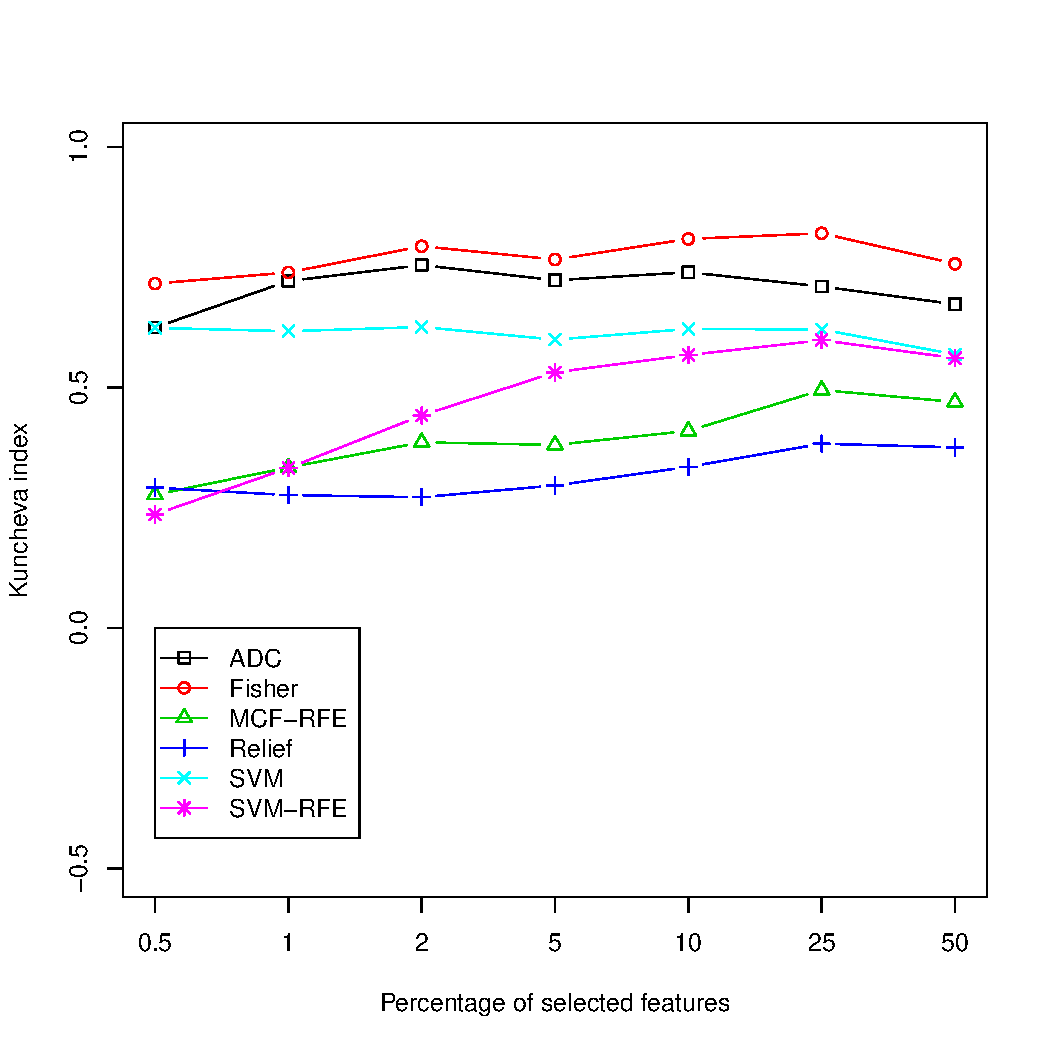
\includegraphics[width=.85\textwidth]{../bachelor/images/nncolon_robustness_kuncheva.pdf}
\caption{Matų atrinkimo gaubtinės žarnos auglio mėginiams stabilumo grafikas pagal Kuncheva indeksą.}
\label{fig:robk_colon}
\end{minipage}
\hspace{0.2cm}
\begin{minipage}[b]{0.47\linewidth}
\centering
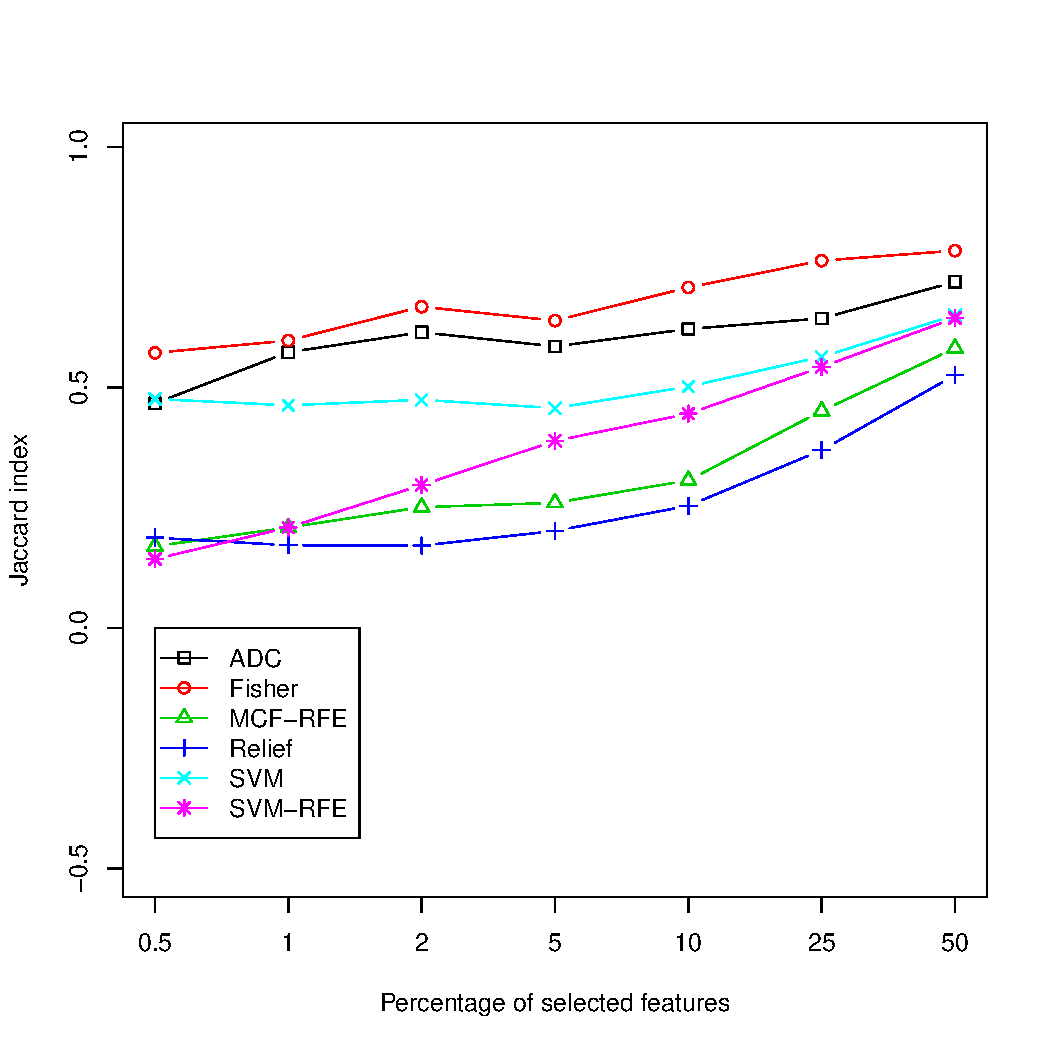
\includegraphics[width=.85\textwidth]{../bachelor/images/nncolon_robustness_jaccard.pdf}
\caption{Matų atrinkimo gaubtinės žarnos auglio mėginiams stabilumo grafikas pagal Jaccard indeksą.}
\label{fig:robj_colon}
\end{minipage}
\hspace{0.2cm}
\begin{minipage}[b]{0.47\linewidth}
\centering
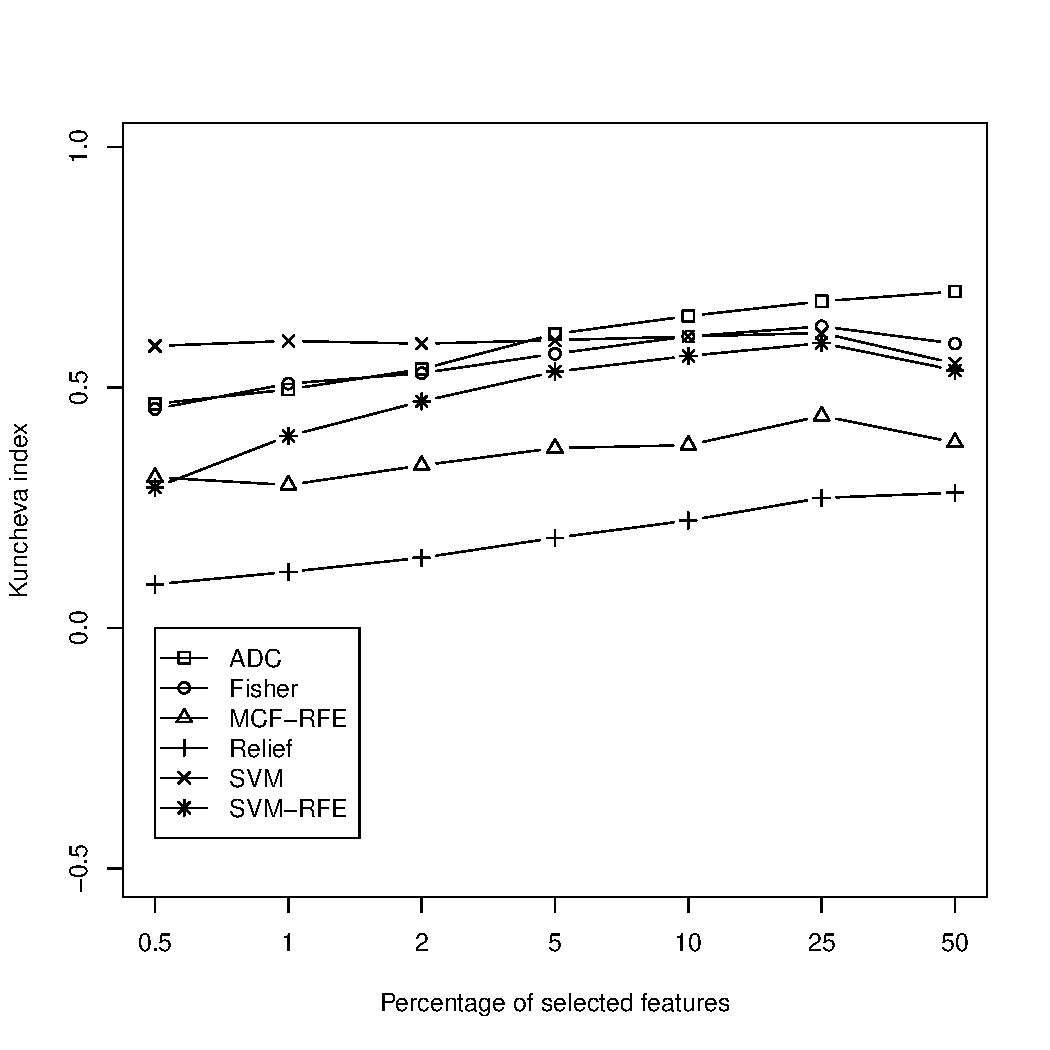
\includegraphics[width=.85\textwidth]{../bachelor/images/nncns_robustness_kuncheva.pdf}
\caption{Matų atrinkimo CNS mėginiams stabilumo grafikas pagal Kuncheva indeksą.}
\label{fig:robk_cns}
\end{minipage}
\hspace{0.2cm}
\begin{minipage}[b]{0.47\linewidth}
\centering
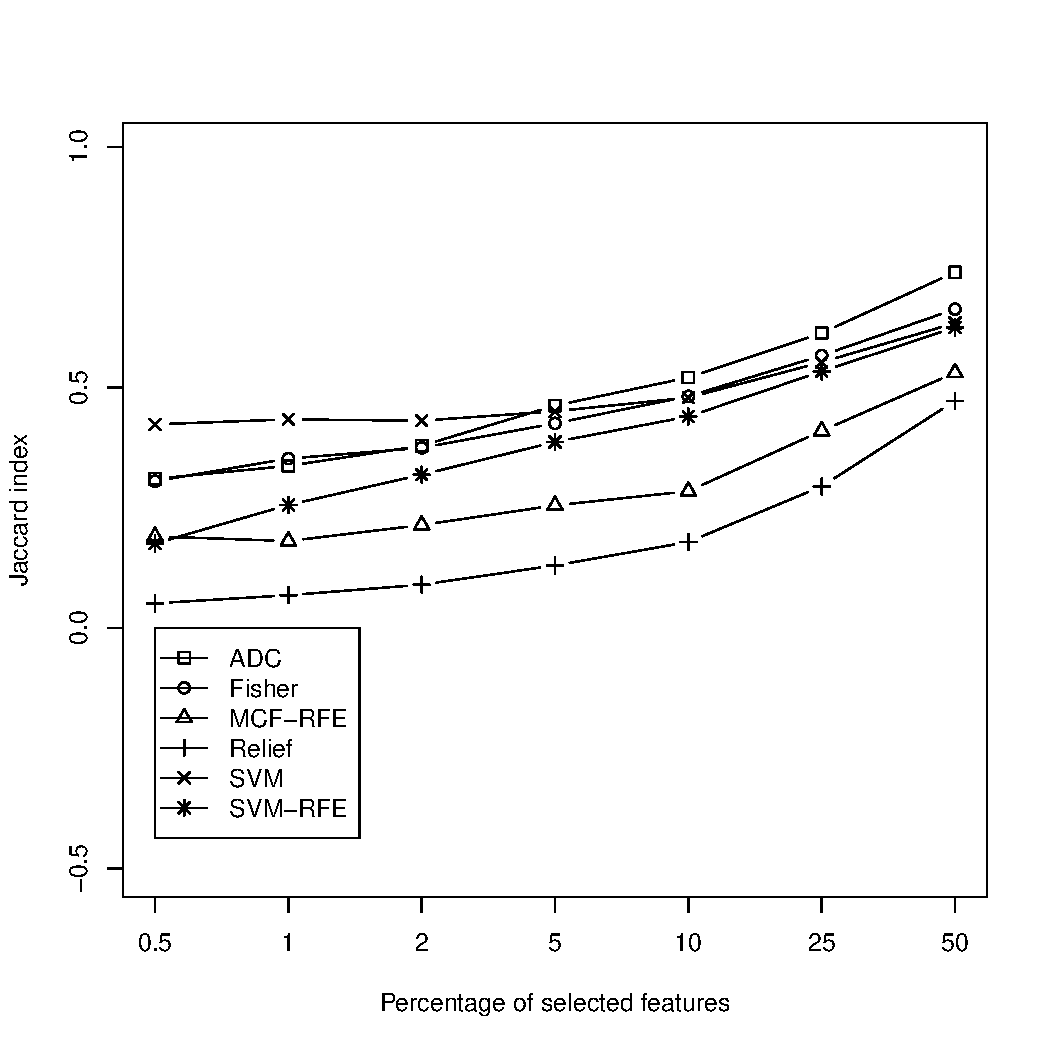
\includegraphics[width=.85\textwidth]{../bachelor/images/nncns_robustness_jaccard.pdf}
\caption{Matų atrinkimo CNS mėginiams stabilumo grafikas pagal Jaccard indeksą.}
\label{fig:robj_cns}
\end{minipage}
\hspace{0.2cm}
\begin{minipage}[b]{0.47\linewidth}
\centering
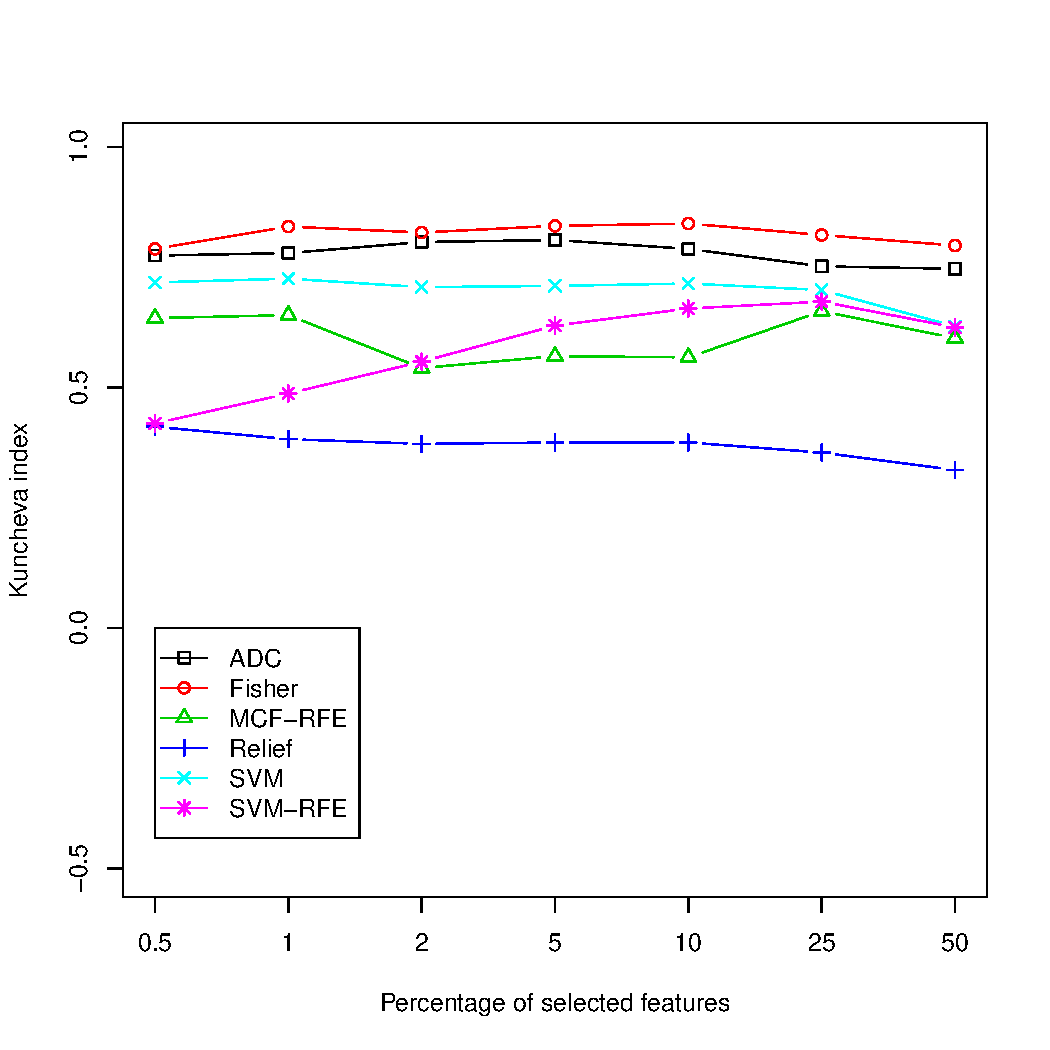
\includegraphics[width=.85\textwidth]{../bachelor/images/prostate_robustness_kuncheva.pdf}
\caption{Matų atrinkimo prostatos mėginiams stabilumo grafikas pagal Kuncheva indeksą.}
\label{fig:robk_prostate}
\end{minipage}
\hspace{0.2cm}
\begin{minipage}[b]{0.47\linewidth}
\centering
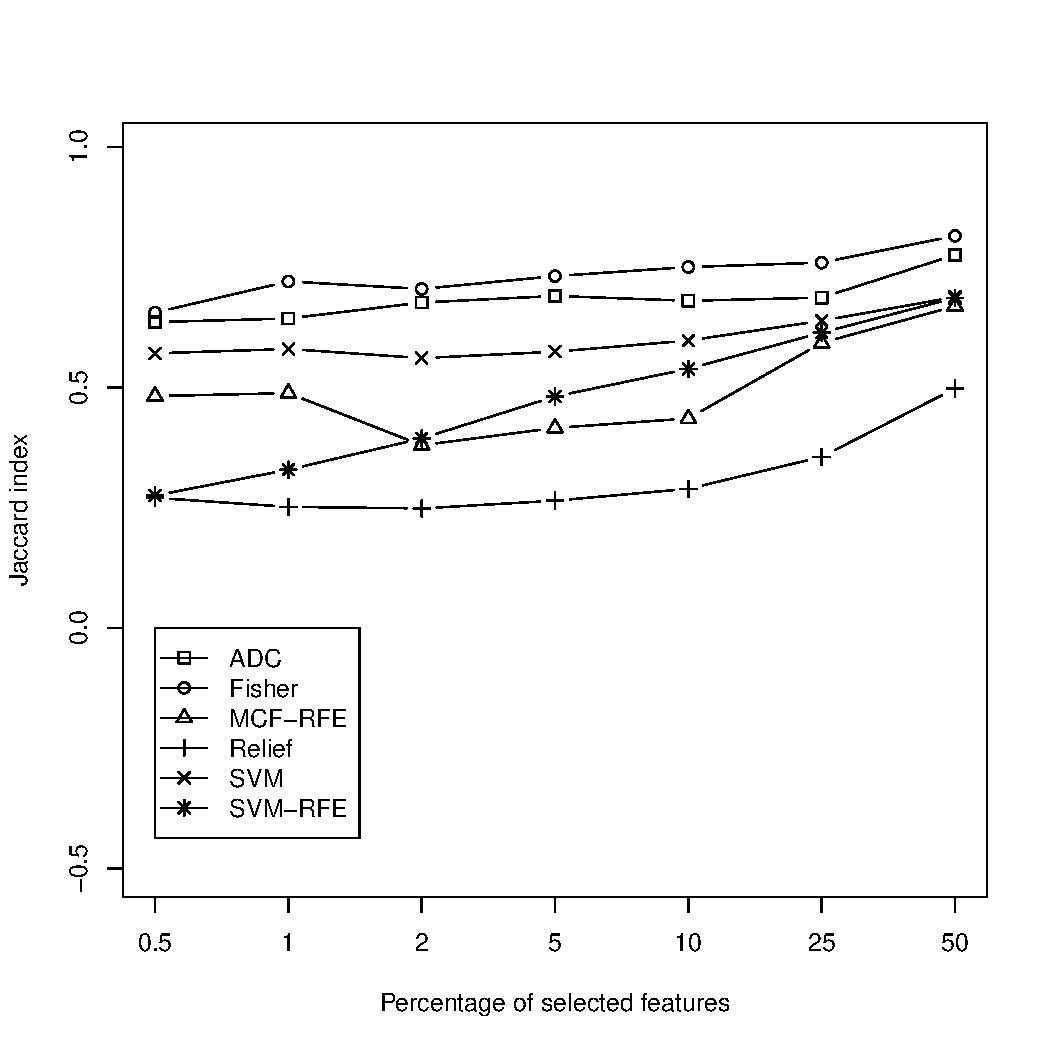
\includegraphics[width=.85\textwidth]{../bachelor/images/prostate_robustness_jaccard.pdf}
\caption{Matų atrinkimo prostatos mėginiams stabilumo grafikas pagal Jaccard indeksą.}
\label{fig:robj_prostate}
\end{minipage}
\end{figure}
Pagal \ref{fig:robk_colon} pav. ir \ref{fig:robj_colon} pav. galima teigti, kad gaubtinės žarnos auglio duomenų rinkinio matus stabiliausiai atrenka \textit{Fisher} įvertis. Mažiausiai stabiliai matus atrenka \textit{Relief} metodas.

Pagal \ref{fig:robk_prostate} pav. ir \ref{fig:robj_prostate} pav. galima teigti, kad prostatos duomenų rinkinio matus stabiliausiai atrenka \textit{Fisher} įvertis. Mažiausiai stabiliai matus atrenka \textit{Relief} metodas.

Apibendrinant matų atrinkimo stabilumo matavimus galima daryti išvadą, kad matų atrinkimo stabilumas priklauso ne tik nuo matų atrinkimo metodo, bet ir nuo duomenų rinkinio, kurio matai yra atrenkami. Lengvai klasifikuojamo prostatos duomenų rinkinio matų atrinkimo stabilumas vidutiniškai yra didesnis nei sunkiai klasifikuojamo CNS duomenų rinkinio. Eksperimentų rezultatai rodo, kad \textit{Relief} matų atrinkimo metodas yra nestabiliausias iš tirtųjų. Gana geru stabilumu pasižymi ADC metodas bei \textit{Fisher} įvertis.
